\documentclass[12pt]{article}
\usepackage[inner=2.0cm,outer=2.0cm,top=2.5cm,bottom=2.5cm]{geometry}
\usepackage{float}
\usepackage{graphicx}
\usepackage{hyperref}
\setlength\voffset{-0.25in}
\setlength\textheight{675pt}

\usepackage{titling}
\setlength{\droptitle}{19em}
\title{CS 3651 - Prototyping Intelligent Devices\\ Project Proposal \\Wall-E}
\author{Names: Nithya Jayakumar, Tri Le}
\date{\today}


\begin{document}
\maketitle

\newpage
\section{Description} % A written description of what you hope to accomplish
    The project aims to construct a functional small-scale robot inspired by Wall-E, with a focus on mobility through the integration of distance sensors. The team envisions utilizing 3D printing technology to manufacture the robot's chassis. Our goal is to meticulously recreate a miniaturized version of Wall-E, achieving a 90\% replica in terms of functionality. While omitting features related to listening and solar panel functions, our primary objective is to develop a fully operational robot. One notable addition is the implementation of a notification system to alert users when the robot's battery reaches a low level. This multifaceted project involves a combination of mechanical design, sensor integration, and programming to bring the mini Wall-E to life.

    \begin{figure}[H]
        \centering
        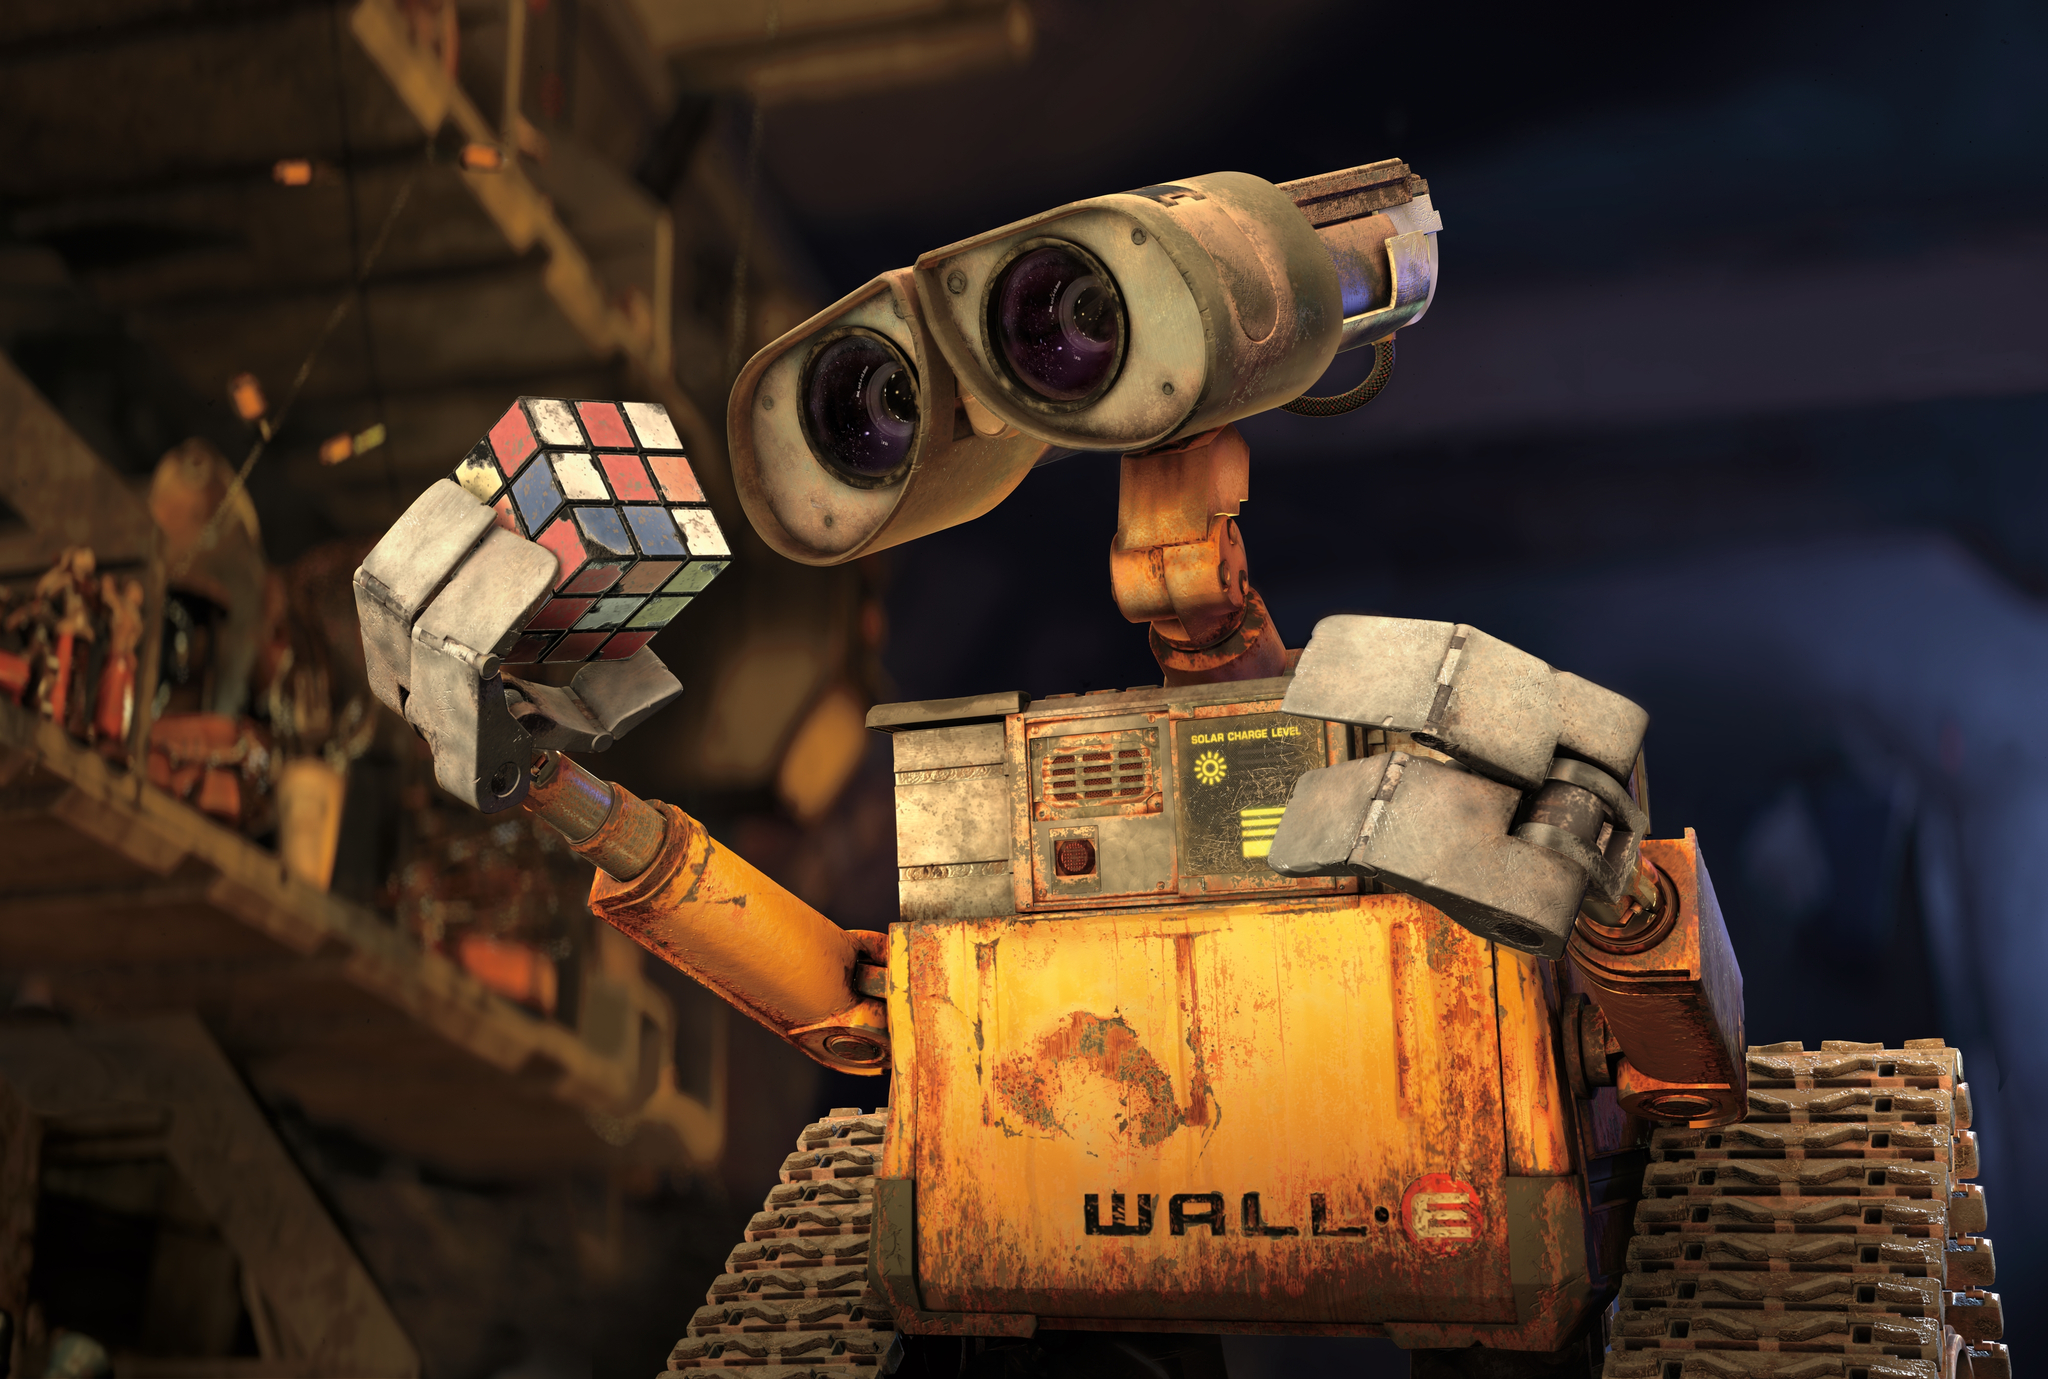
\includegraphics[width=0.6\linewidth]{wall-eee.jpg}
        \caption{Wall-E in Movie.}
    \end{figure}

\section{Resources} % Links to resources you’ve found so far
\begin{itemize}
    \item[1.] DIY fully functional mini Wall-E using Arduino Nano - \href{https://www.youtube.com/watch?v=iaqVNqsvQwI}{link} \& \href{https://www.youtube.com/watch?v=Cqv2w0qYf-s}{link} \\\\
        This resource provides insights into the required parts and the overall functioning of a mini Wall-E using Arduino Nano. Our project will follow a similar concept, but with the added feature of autonomous movement.
    \item[2.] 3D printed Wall-E replica tutorial - \href{https://www.youtube.com/watch?v=SJ2odjtOjxY}{link} \\\\
        This tutorial guides the 3D printing process for a Wall-E replica. We plan to modify the provided CAD file to adapt the size and integrate our specific components for a smaller version of Wall-E.
    \item[3.] 3D printed Wall-E with a list of components required and parts to make the robot fully functioning - \href{https://wired.chillibasket.com/3d-printed-wall-e/}{link} \& \href{https://youtu.be/ZRK9f4FZlD8}{link} \\\\
        This resource offers valuable information on the components required for a fully functioning 3D printed Wall-E. We will adapt the information to fit our project's specifications, modifying motor sizes, battery sizes, and integrating sensors for autonomous movement.
    \item[4.] Wall-E communication - \href{https://blog.arduino.cc/2021/07/03/build-your-own-adorable-talking-wall-e-robot/}{link} \\\\
        This resource focuses on Wall-E's communication abilities, including listening to commands and playing music. We plan to incorporate a similar communication system into our mini Wall-E for user interaction.
\end{itemize}


\section{Design} % A tentative high-level design
The high-level design of the Wall-E robot encompasses several key components, each contributing to the overall functionality and appearance of the robot.
\begin{itemize}
    \item \textbf{Brain - Core Functionality} \\
    The brain of the Wall-E robot is the central unit responsible for controlling its movements, obstacle avoidance, and overall functionality. This component will utilize the following key elements:
    \begin{itemize}
        \item \textbf{Arduino Nano:} Serving as the primary microcontroller, the Arduino Nano will execute the robot's code, coordinating various actions and responses.
    
        \item \textbf{Bluetooth Chip:} Enabling wireless communication, the Bluetooth chip allows for remote control and potential voice command input, facilitating user interaction.
        
        \item \textbf{TOF (Time-of-Flight) Distance Sensor:} This sensor is crucial for obstacle detection and avoidance, ensuring the robot can navigate its environment safely.
        
        \item \textbf{H-Bridge:} Responsible for controlling the DC motors that drive the robot's movement, the H-Bridge facilitates precise control over speed and direction.
        \begin{figure}[H]
            \centering
            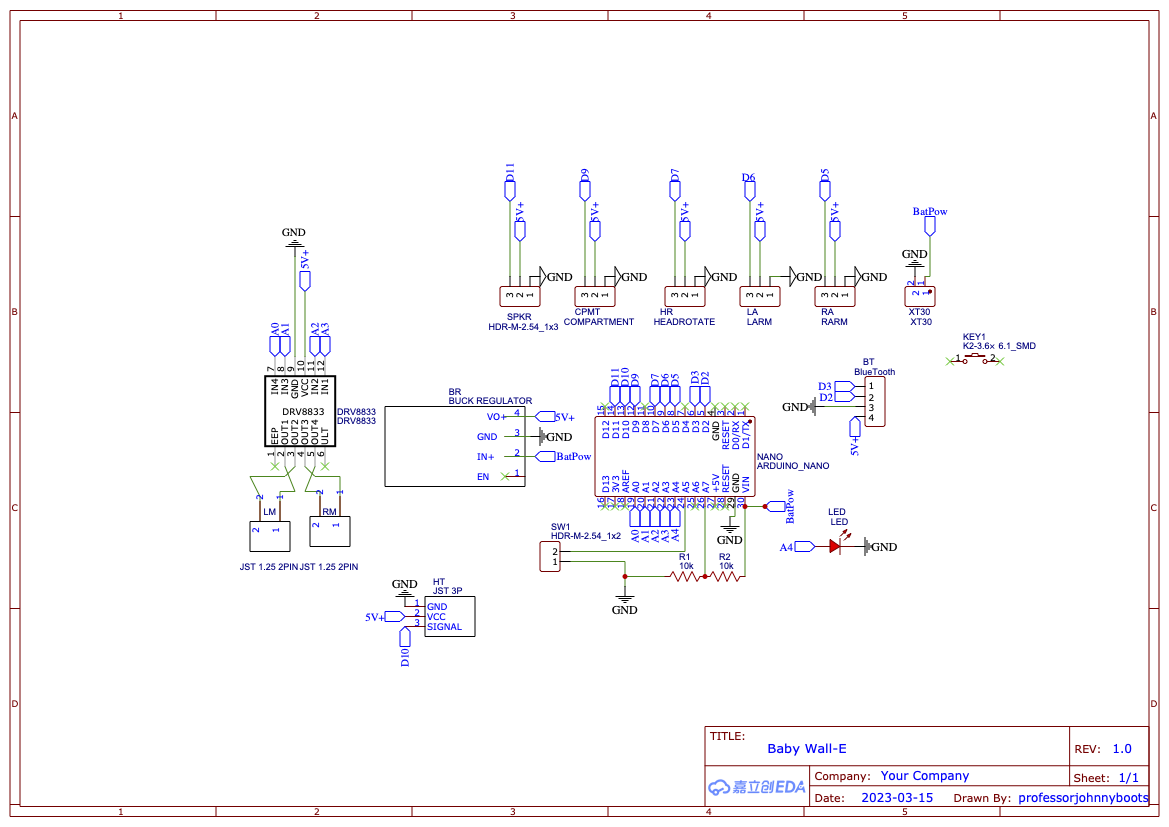
\includegraphics[width=0.5\linewidth]{Schematic_Baby_Wall-E_Control_Board.png}
            \caption{Wall-E Control Board/Brain}
        \end{figure}
    \end{itemize}
    The code executed by the Arduino Nano will include algorithms for movement, obstacle detection, and interaction with other components, ensuring a seamless and intelligent behavior.
    \item \textbf{Skeleton - Physical Movements}\\
    The skeleton of the Wall-E robot refers to its physical structure, incorporating movable components that bring the robot to life. This includes:
    \begin{itemize}
        \item \textbf{Servos:} Used to control the movement of the robot's eyes, neck (up and down), head rotation, and arms, servos add dynamic and expressive qualities to the robot's appearance.
        
        \item \textbf{DC Motors:} These motors drive the wheels, allowing the robot to move forward, backward, and turn in response to commands from the brain.
        
        \item \textbf{Battery:} Providing power to the motors, servos, and other electronic components, the battery ensures sustained operation.
        
        \item \textbf{Speaker:} The speaker is integrated for audio output, enabling the robot to produce sounds, potentially including Wall-E's signature song.
    \end{itemize}
    \begin{figure}[H]
        \centering
        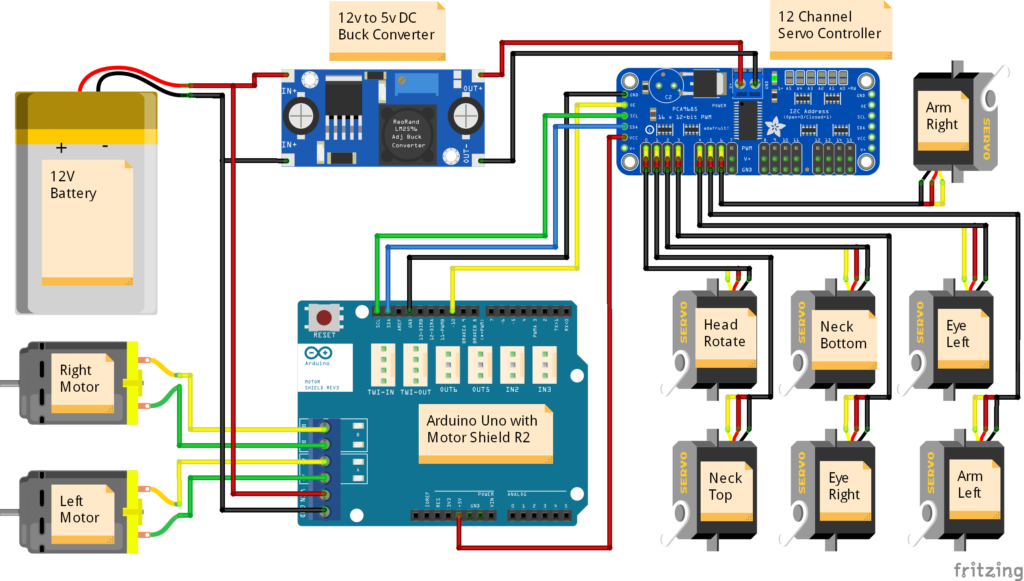
\includegraphics[width=0.5\linewidth]{Wall-E-Circuit-Diagram-1024x581.png}
        \caption{Skeleton diagram of the Wall-E robot. Note: Due to some parts changes, this diagram may not be fully accurate. It serves the purpose of illustrating the required components and their connections.}
    \end{figure}
    
    Assembling this skeleton involves careful placement and connection of components, considering balance and stability to achieve fluid and coordinated movements.

    \item \textbf{Exterior - The "Skin"}\\
    The exterior, or "skin," represents the outer appearance of the Wall-E robot. While this is a challenging aspect, it contributes significantly to the project's aesthetics. The team plans to use 3D printing based on tutorials and CAD models, modifying them to fit the scaled-down version of Wall-E.
    \begin{figure}[H]
        \centering
        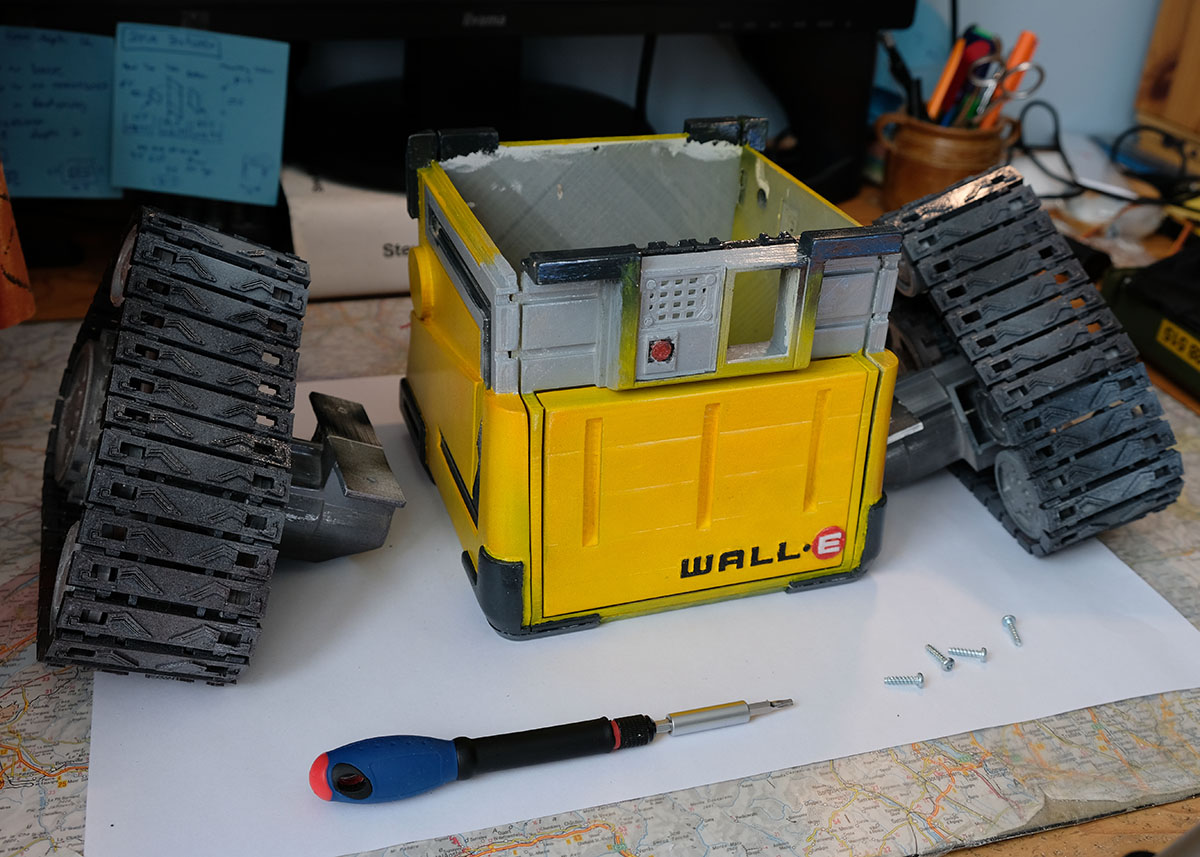
\includegraphics[width=0.5\linewidth]{Assembly_Body_and_Wheels.jpg}
        \caption{Example of 3D Printed Parts of Wall-E Robot.}
    \end{figure}
    However, due to limited experience with CAD, creating the exterior is marked as a "stretch goal" for the project, acknowledging potential challenges and the need for additional learning and resources.
    \begin{figure}[H]
        \centering
        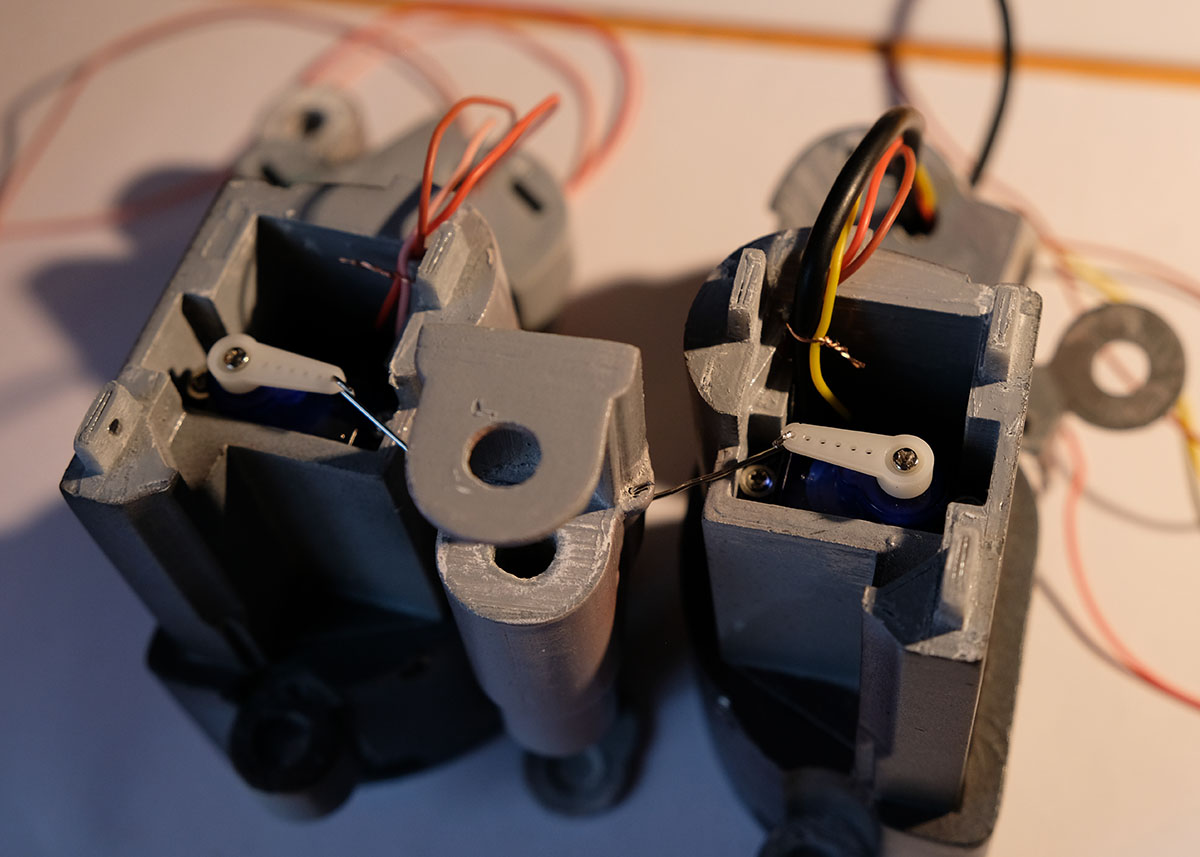
\includegraphics[width=0.5\linewidth]{Assembly_Eyes_Servos.jpg}
        \caption{Example of 3D-printed WALL-E eyes with servos to control left and right eye movements, including sensors in both eyes.}
    \end{figure}

    \item \textbf{Voice Command (Stretch Goal)}\\
    If time allows, the team aims to implement a voice command feature, enabling the Wall-E robot to respond to spoken commands. This feature adds an interactive and user-friendly dimension to the robot's capabilities. The voice command system may include recognizing phrases like "move left," "move right," "stop," "forward," "backward," and specific voice commands for the robot's name and song playback.
    
    This feature is designated as a "stretch goal," recognizing its complexity and potential for additional development beyond the primary project objectives.
    
    In summary, the high-level design breaks down the Wall-E robot into its core components, addressing both functional and aesthetic aspects while also acknowledging potential challenges and stretch goals.
\end{itemize}


\subsection{Wall-E Parts Details}
% Parts that you’re considering using. If you are planning to use some major parts from around the lab, this might be a good time to mention them to ensure you’re not going to conflict with another group.
\begin{itemize}
    \item Arduino Nano - \href{https://www.amazon.com/Arduino-A000005-ARDUINO-Nano/dp/B0097AU5OU/ref=asc_df_B0097AU5OU/?tag=hyprod-20&linkCode=df0&hvadid=241907595991&hvpos=&hvnetw=g&hvrand=1030222966127056408&hvpone=&hvptwo=&hvqmt=&hvdev=c&hvdvcmdl=&hvlocint=&hvlocphy=9060222&hvtargid=pla-559564017483&psc=1&mcid=070a72770c7e334fa02abb503757b8a1&gclid=Cj0KCQiA84CvBhCaARIsAMkAvkIJoyGS0PcNJItudCSnEclnk1MBDUQ7vMJqO9LYnJ1i24tnsd1vVvsaAh1QEALw_wcB}{link} [x1]
    \item HM-10 Bluetooth Chip - \href{https://www.amazon.com/DSD-TECH-Bluetooth-iBeacon-Arduino/dp/B06WGZB2N4?crid=2864IU5C7C4LI&keywords=hm-10+bluetooth+module&qid=1680999661&sprefix=hm-10+b,aps,211&sr=8-1-spons&psc=1&spLa=ZW5jcnlwdGVkUXVhbGlmaWVyPUFFMVI0RzdINktUR0omZW5jcnlwdGVkSWQ9QTA3MTEwNTQxWkNYRFhJWEdJSlBSJmVuY3J5cHRlZEFkSWQ9QTA2OTcyODkzMzdSV0FSMkhKRkdLJndpZGdldE5hbWU9c3BfYXRmJmFjdGlvbj1jbGlja1JlZGlyZWN0JmRvTm90TG9nQ2xpY2s9dHJ1ZQ%3D%3D&linkCode=sl1&tag=professorboot-20&linkId=51ea8e01ed875db9c550dfc3b298172f&language=en_US&ref_=as_li_ss_tl}{link} [x1]
    \item H-Bridge [x1]
    \item AA battery [x4]
    \item Buck Converter - \href{https://www.amazon.com/gp/product/B08Y674Z6F?ie=UTF8&th=1&linkCode=sl1&tag=professorboot-20&linkId=9f7b55a9e0472ae92cea90d04bb54435&language=en_US&ref_=as_li_ss_tl}{link} [x1]
    \item Servos - \href{https://www.amazon.com/dp/B098FG3LJF?th=1&linkCode=sl1&tag=professorboot-20&linkId=9cd9bc0acb06cb36fc01f502b2cd1ff1&language=en_US&ref_=as_li_ss_tl}{link} [x5]
    \item 3V-6V DC Motors - \href{https://www.amazon.com/dp/B09WMJJ8SF?psc=1&linkCode=sl1&tag=professorboot-20&linkId=741cfbc8d0840160116efdb36d687af6&language=en_US&ref_=as_li_ss_tl}{link} [x2]
    \item Ultrasonic Sensor [x2]
    \item Others (bolt, nut, wire, resistors, lens, led, paper clips, etc)
\end{itemize}

\subsubsection{Helpful Resources/Tutorial} % Don't just tell us that you found a tutorial or part, give us a link to it!
\begin{itemize}
    \item \textbf{Wall-E Resources}
    \begin{itemize}
        \item[1] \href{https://www.youtube.com/watch?v=Cqv2w0qYf-s}{How To Make a Baby Wall-E Robot} 
        \item[2] \href{https://wired.chillibasket.com/3d-printed-wall-e/}{3D Printed Wall-E} 
        \item[3] \href{https://drive.google.com/drive/folders/1AiicgyjlS-KWhi7NfhnoCsdB6uxxlqcq?usp=sharing}{3D Wall-E CAD STEP file} 
        \item[4] \href{https://wired.chillibasket.com/wp-content/uploads/2019/06/Wall-E-List-of-Parts.pdf}{3D Printed Wall-E - List of all components }
        \item[5] \href{https://blog.arduino.cc/2021/07/03/build-your-own-adorable-talking-wall-e-robot/}{Build an adorable, talking Wall-E robot}
        \item[6] \href{https://www.youtube.com/watch?v=xO5_3SjEhS4}{Laser vs Ultrasonic - TOF10120 vs. HC-SR04}
        \item[7] \href{https://www.thingiverse.com/thing:5957438/files}{Baby Wall-E (Fully Functional) - 3D files}
    \end{itemize}
    
    \item \textbf{CAD Modeling for 3D Printing Resources}
    \begin{itemize}
        \item[1] \href{https://www.youtube.com/watch?v=IUoTKbGAlhk}{Getting Started with CAD Modeling for 3D Printing}
        \item[2] \href{https://www.youtube.com/watch?v=1QNVyMBV0fM}{CAD TUTORIAL : FreeCAD Beginner [EASY GUIDE]}
        \item[3]  \href{https://www.youtube.com/watch?v=vK-O7hwKYYQ}{Tutorial - Step File Modeling Techniques}
        \item[4] \href{https://www.youtube.com/watch?v=Ae5O7j-hFwg}{FreeCAD for Beginners pt.7 - Importing .STEP files and Scaling}
    \end{itemize}
    
    \item \textbf{TOF Distance Sensor OR Ultrasonic Sensor}
    \begin{itemize}
        \item[1] \href{https://www.youtube.com/watch?v=VnSfw9ynemc}{Arduino Laser Time-of-Flight Sensor Touch-Free Input Tutorial}
        \item[2] \href{https://www.youtube.com/watch?v=ii5ofdo_968}{ESP8266 and Arduino Robotics: Measuring Distances w/ Ultrasonic Sensor HC-SR04 | WHEEL-E Robot}
        \item[3] \href{https://www.youtube.com/watch?v=nUas-A0THDo}{Obstacle Avoiding Robot Car Using An Arduino} 
        \item[4] \href{https://www.youtube.com/watch?v=4X_EjUZp2c0}{ROOM MAPPING Arduino Robot}
        \item[5] \href{https://www.youtube.com/watch?v=yAV5aZ0unag}{How To Make Arduino Human Following Robot}
        \item[6] \href{https://www.instructables.com/Obstacle-Avoiding-Robot-Arduino-1/#}{Obstacle Avoiding Robot (Arduino)} 
    \end{itemize}
\end{itemize}

\section{Expectations/Goals} % What you would expect to accomplish to earn an ‘A’ on the project. Consider listing out a minimum set of features you're planning to implement, plus any "stretch goals". We’ll work with you to adjust these (if needed) so that each team has realistic but challenging enough goals.

The team's goal is to build a fully functional WALL-E robot. However, as mentioned, the exterior part of the WALL-E robot will be optional (a stretch goal) due to the difficulty and limited 3D printing skills. The project of building a fully functional robot is already challenging. The challenges include obstacle avoidance, how motors/wheels will turn/run, how the ultrasonic screening/TOF sensor will work, and how to make it work, including mapping.

The team believes that to earn an 'A' for this project, they must achieve the following:

\begin{itemize}
    \item[a] Implement a working robot "brain" with code that makes the robot function similarly to the WALL-E robot.
    \item[b] Ensure the ultrasonic/TOF sensor detects obstacles.
    \item[c] Make the wheels turn, run, and stop based on the information gathered by the sensor.
    \item[d] Implement robot mapping.
    \item[e] Achieve a partially completed WALL-E exterior (not fully perfect).
\end{itemize}

However, the team recognizes that to earn a perfect 'A' for this project, they need to have a fully completed 3D printed exterior of the WALL-E robot.\\

Additionally, the team believes there can be a bonus for the project if they are able to make the robot a rechargeable hub. The robot would autonomously return to recharge its battery when low, and the charging hub would utilize a solar panel (similar to the movie). WALL-E should also be able to communicate by listening to voice commands for turning, running, stopping, moving backward, playing a song, and saying its name when asked.

\section{Mid-Project Deliverable}
% A hard deliverable for the mid-project review. Select one (or more) critically important parts of your project, and get it working. This gives us a chance to help you re-target your project if you hit a big roadblock.

For the mid-project deliverable, the team aims to accomplish the following:

\begin{itemize}
    \item[1] Complete the construction of the robot's brain, including wiring, soldering parts, and assembling the components.
    \item[2] Partially 3D print the robot's exterior.
    \item[3] Enable the robot to move left, right, and stop using sensors, and ensure it can avoid obstacles.
    \item[4] Fully complete the robot's skeleton, including the integration of the battery.
    \item[5] Ensure that all servos, motors, and sensors work as expected. 
\end{itemize}

\end{document}